% !TeX program = xelatex
\documentclass[a4paper,10pt]{article}

% ============================================================================
% សន្លឹកកិច្ចការសិស្សបំពេញចន្លោះ ស-ខ្មៅ និងប្លង់ក្ដារខៀន/ចម្លើយគ្រូ (គ្មាន LCD / គ្មានកន្ត្រៃ)
% មេរៀនទី២ (៤.)៖ ការបំបែកមួយចំនួនជាផលគុណកត្តាបឋម — ត្រូវគ្នា ១០០% នឹង LS_Plan_DIV24.tex
% ============================================================================
\usepackage[a4paper, left=1.0cm, right=1.0cm, top=0.75cm, bottom=1.00cm, footskip=0.52cm]{geometry}
\usepackage{amsmath}
\usepackage{unicode-math}
\usepackage{fontspec}
\usepackage{array, colortbl}
\usepackage[table]{xcolor}
\usepackage{enumitem}
\usepackage{pifont}
\usepackage{fancyhdr}
\usepackage{lastpage}
\usepackage{tikz}
\usepackage[most]{tcolorbox}
\usetikzlibrary{calc, arrows.meta, decorations.pathreplacing, positioning, babel}

\makeatletter
\let\@expl@@@mark@update@singlecol@structures@@\relax
\makeatother

\providecommand{\NGSFindFonts}{%
  \IfFileExists{C:/Windows/Fonts/cambria.ttc}{%
    \def\NGSSysPath{C:/Windows/Fonts/}%
    \def\NGSUserPath{C:/Users/KIT/AppData/Local/Microsoft/Windows/Fonts/}%
  }{%
    \IfFileExists{./fonts/KhmerOSsiemreap.ttf}{\def\NGSSysPath{./fonts/}\def\NGSUserPath{./fonts/}}{%
    \IfFileExists{../fonts/KhmerOSsiemreap.ttf}{\def\NGSSysPath{../fonts/}\def\NGSUserPath{../fonts/}}{%
    \IfFileExists{../../fonts/KhmerOSsiemreap.ttf}{\def\NGSSysPath{../../fonts/}\def\NGSUserPath{../../fonts/}}{%
    \IfFileExists{../../../fonts/KhmerOSsiemreap.ttf}{\def\NGSSysPath{../../../fonts/}\def\NGSUserPath{../../../fonts/}}{%
    \IfFileExists{../../../../fonts/KhmerOSsiemreap.ttf}{\def\NGSSysPath{../../../../fonts/}\def\NGSUserPath{../../../../fonts/}}{%
    \IfFileExists{../../../../../fonts/KhmerOSsiemreap.ttf}{\def\NGSSysPath{../../../../../fonts/}\def\NGSSysPath{../../../../../fonts/}}{%
    \IfFileExists{../../../../../../fonts/KhmerOSsiemreap.ttf}{\def\NGSSysPath{../../../../../../fonts/}\def\NGSUserPath{../../../../../../fonts/}}{%
      \def\NGSSysPath{../../../../../../../fonts/}\def\NGSUserPath{../../../../../../../fonts/}%
    }}}}}}}%
  }%
}
\NGSFindFonts

\setmathfont[Path={\NGSSysPath}, FontIndex=1, Scale=1.02]{cambria.ttc}
\defaultfontfeatures{Ligatures=TeX}

\setmainfont[
  Path={\NGSUserPath}, Extension=.ttf, Script=Khmer,
  BoldFont={KhmerOSsiemreap}, BoldFeatures={FakeBold=1.8},
  ItalicFont={KhmerOSsiemreap}, ItalicFeatures={FakeSlant=0.25},
  BoldItalicFont={KhmerOSsiemreap}, BoldItalicFeatures={FakeBold=1.8, FakeSlant=0.25}
]{KhmerOSsiemreap}

\newfontfamily\muol[Path={\NGSUserPath}, Extension=.ttf, Script=Khmer]{KhmerOSmuollight}
\newfontfamily\TimesEn[Path={\NGSSysPath}, Extension=.ttf, BoldFont={timesbd}, ItalicFont={timesi}, BoldItalicFont={timesbi}]{times}
\newfontfamily\CalibriFont[Path={\NGSSysPath}, Extension=.ttf]{calibri}

\XeTeXlinebreaklocale "km"
\XeTeXlinebreakskip = 0pt plus 1pt minus 0.1pt

\definecolor{panelgray}{gray}{0.94}
\definecolor{headgray}{gray}{0.85}

\pagestyle{fancy}
\fancyhf{}
\renewcommand{\headrulewidth}{0pt}
\fancyfoot[L]{\fontsize{7.4pt}{9.5pt}\selectfont អនុវិទ្យាល័យព្រះក្រសាំង \en{|} គ្រូ៖ ហុក ប៊ុនថែន \en{|} មេរៀនទី២ (៤.) ការបំបែកមួយចំនួនជាផលគុណកត្តាបឋម \en{|} ថ្ងៃចន្ទ ទី១៦ ខែវិច្ឆិកា ឆ្នាំ២០២៦}
\fancyfoot[R]{\fontsize{7.8pt}{10pt}\selectfont ទំព័រ \en{\thepage\ / \pageref{LastPage}}}

\setlength{\parindent}{0pt}
\setlength{\parskip}{0pt}
\setlength{\tabcolsep}{4pt}
\newcolumntype{L}[1]{>{\raggedright\arraybackslash}p{#1}}
\newcolumntype{C}[1]{>{\centering\arraybackslash}p{#1}}

\newcommand{\en}[1]{{\TimesEn #1}}
\newcommand{\enbf}[1]{{\TimesEn\bfseries #1}}
\newcommand{\unit}[1]{\,\text{\en{#1}}}
\newcommand{\cnum}[1]{\mbox{\fontsize{10pt}{12pt}\selectfont\ding{\numexpr181+#1\relax}}}
\newcommand{\chkbox}{\tikz[baseline=-0.15ex]\draw[black, line width=0.85pt, fill=white] (0,0) rectangle (0.24cm,0.24cm);}
\newcommand{\ansbox}[1][1.75cm]{\,\tikz[baseline=-0.65ex]\draw[black, line width=0.65pt, fill=white] (0,0) rectangle (#1, 0.42cm);\,}
\newcommand{\dotline}[1][2.2cm]{\makebox[#1]{\dotfill}}

\newcommand{\pagebanner}[2]{%
  \begin{tcolorbox}[
    enhanced, sharp corners, colback=headgray, colframe=black,
    boxrule=1.05pt, boxsep=1pt, top=2.5pt, bottom=2.5pt, left=6pt, right=6pt,
    after skip=3.5pt
  ]
    {\muol\fontsize{9.0pt}{13.2pt}\selectfont #1}\hfill{\fontsize{8.0pt}{11.2pt}\selectfont\textbf{#2}}
  \end{tcolorbox}%
}

\newcommand{\secstrip}[2]{%
  \vspace{3pt}%
  \begin{tcolorbox}[
    enhanced, sharp corners, colback=panelgray, colframe=black,
    boxrule=0.8pt, boxsep=0.8pt, top=2pt, bottom=2pt, left=5pt, right=5pt,
    after skip=3pt
  ]
    {\muol\fontsize{8.5pt}{12.2pt}\selectfont #1}\hfill{\fontsize{7.8pt}{10.8pt}\selectfont\textit{#2}}
  \end{tcolorbox}%
}

\begin{document}
\fontsize{9.5pt}{14.5pt}\selectfont

% ============================================================================
% ទំព័រទី ១៖ សន្លឹកកិច្ចការសិស្ស (ផ្នែកមុខ៖ E1 -> E2 -> E3)
% ============================================================================
\pagebanner{សន្លឹកកិច្ចការសិស្ស \enbf{(}៤\enbf{.} ការបំបែកមួយចំនួនជាផលគុណកត្តាបឋម\enbf{)} \enbf{--} ផ្នែកមុខ}{ថ្នាក់ទី៧ \en{|} សៀវភៅគោល ទំ.២០}

\begin{tcolorbox}[
  enhanced, sharp corners, colback=white, colframe=black,
  boxrule=0.8pt, boxsep=1.5pt, top=3.5pt, bottom=3.5pt, left=5pt, right=5pt,
  after skip=4pt
]
  \fontsize{9.0pt}{13.0pt}\selectfont
  \textbf{ឈ្មោះសិស្ស៖} \dotline[4.3cm] \quad
  \textbf{សមាជិកក្រុម៖} \dotline[4.3cm] \quad
  \textbf{ថ្នាក់ទី៖} ៧\dotline[0.9cm] \quad
  \textbf{ក្រុមទី៖} \dotline[1.0cm]
\end{tcolorbox}

% --- E1 Engage ---
\secstrip{ផ្នែកទី ១ \enbf{(E1 - Engage)} ៖ បេសកកម្មអន្ទាក់ឈប់ត្រឹមកត្តាមិនបឋម}{រយៈពេល ៣ នាទី (គូស \ding{51} ក្នុង \chkbox)}

\begin{tcolorbox}[
  enhanced, sharp corners, colback=white, colframe=black,
  boxrule=0.8pt, boxsep=2pt, top=4pt, bottom=4pt, left=6pt, right=6pt
]
  គេឱ្យបំបែកចំនួន $36$ ជា\textbf{ផលគុណនៃកត្តាបឋម}៖\\[2.5pt]
  $\bullet$ \chkbox\ \textbf{សិស្ស ក៖} «$36 = 4 \times 9$ — បំបែកជាផលគុណកត្តាបឋមរួចហើយ!»\\[2pt]
  $\bullet$ \chkbox\ \textbf{សិស្ស ខ៖} «$4$ និង $9$ មិនទាន់ជាចំនួនបឋមទេ ត្រូវបំបែកបន្ត $4=2\times 2$ និង $9=3\times 3$ ទើបបាន $36 = 2^2 \times 3^2$!»
\end{tcolorbox}

\vfill

% --- E2 Explore ---
\secstrip{ផ្នែកទី ២ \enbf{(E2 - Explore)} ៖ ប្រៀបធៀបវិធីទី 1 (ចែកឈរ) និងវិធីទី 2 (ដ្យាក្រាមដើមឈើ) (ទំ.២០)}{រយៈពេល ១១ នាទី}

\textbf{សកម្មភាព ១ (\en{E2-A} — ៥.៥ នាទី)៖ បំបែកចំនួន $30$ តាមវិធីទាំងពីរ (សៀវភៅគោល ទំ.២០)}

\begin{tcolorbox}[
  enhanced, sharp corners, colback=white, colframe=black,
  boxrule=0.8pt, boxsep=2.5pt, top=4pt, bottom=4pt, left=6pt, right=6pt
]
  \begin{minipage}[t]{0.47\textwidth}
    \textbf{១) វិធីទី 1៖ ចែកឈរនឹងបឋមតូចបំផុត}\\[3pt]
    \hspace*{0.8cm}$30 \div 2 =$ \dotline[1.1cm]\\[2pt]
    \hspace*{0.8cm}$15 \div$ \dotline[0.8cm] $= 5$\\[2pt]
    \hspace*{1.0cm}$5 \div$ \dotline[0.8cm] $= 1$\\[3pt]
    ដូចនេះ $30 =$ \dotline[0.8cm] $\times$ \dotline[0.8cm] $\times$ \dotline[0.8cm] ។
  \end{minipage}\hfill
  \vrule width 0.6pt\hfill
  \begin{minipage}[t]{0.49\textwidth}
    \textbf{២) វិធីទី 2៖ ដ្យាក្រាមដើមឈើ (គូសរង្វង់ចុងមែកបឋម)}\\[3pt]
    $\bullet$ មែកទី១៖ $30 = 2 \times 15 = 2 \times ($ \dotline[0.8cm] $\times$ \dotline[0.8cm] $)$\\[3pt]
    $\bullet$ មែកទី២៖ $30 = 5 \times 6 = 5 \times ($ \dotline[0.8cm] $\times$ \dotline[0.8cm] $)$\\[3pt]
    រៀបពីតូចទៅធំបាន៖ $30 =$ \ansbox[3.4cm] ដូចគ្នា!
  \end{minipage}
\end{tcolorbox}

\vspace{4pt}
\textbf{សកម្មភាព ២ (\en{E2-B} — ៥.៥ នាទី)៖ បំបែកចំនួន $72$ និងសរសេរជាទម្រង់ស្វ័យគុណ}

\begin{tcolorbox}[
  enhanced, sharp corners, colback=white, colframe=black,
  boxrule=0.8pt, boxsep=2.5pt, top=4.5pt, bottom=4.5pt, left=6pt, right=6pt
]
  \begin{minipage}[t]{0.48\textwidth}
    \textbf{១) តាមចែកឈរបន្តបន្ទាប់៖}\\[2.5pt]
    $72 \div 2 =$ \dotline[0.9cm] $\to \div 2 =$ \dotline[0.9cm]\\[2.5pt]
    $\to \div 2 =$ \dotline[0.9cm] $\to \div 3 =$ \dotline[0.9cm] $\to \div 3 = 1$\\[3pt]
    ផលគុណលាត៖ $72 = 2 \times 2 \times 2 \times 3 \times 3$
  \end{minipage}\hfill
  \vrule width 0.6pt\hfill
  \begin{minipage}[t]{0.48\textwidth}
    \textbf{២) តាមដ្យាក្រាមដើមឈើ ($72 = 8 \times 9$)៖}\\[2.5pt]
    $\bullet$ បំបែក $8 =$ \dotline[0.7cm] $\times$ \dotline[0.7cm] $\times$ \dotline[0.7cm]\\[2.5pt]
    $\bullet$ បំបែក $9 =$ \dotline[0.8cm] $\times$ \dotline[0.8cm]\\[3pt]
    \textbf{ទម្រង់ស្វ័យគុណ៖} $72 =$ \ansbox[2.8cm] ($8\times 9 =$ \dotline[0.9cm])
  \end{minipage}
\end{tcolorbox}

\vfill

% --- E3 Explain ---
\secstrip{ផ្នែកទី ៣ \enbf{(E3 - Explain)} ៖ វិធានទូទៅ សម្គាល់អំពី $1$ និងធនាគារហេតុផល \enbf{B\&W}}{រយៈពេល ៦ នាទី}

\begin{tcolorbox}[
  enhanced, sharp corners, colback=white, colframe=black,
  boxrule=0.85pt, boxsep=2.5pt, top=4pt, bottom=4pt, left=6pt, right=6pt
]
  $\bullet$ \textbf{ជាទូទៅ (ទំ.២០)៖} គ្រប់ចំនួនមិនបឋមទាំងអស់ អាចសរសេរជា \dotline[4.2cm] បានតែមួយបែបគត់ (បើរៀបកត្តាបឋមពីតូចទៅធំ) ។\\[2.5pt]
  $\bullet$ \textbf{សម្គាល់៖} គេ\textbf{មិនដាក់ចំនួន \dotline[0.9cm]} ក្នុងផលគុណកត្តាបឋមឡើយ ព្រោះវាមិនមែនជាចំនួនបឋម!\\[3pt]
  \tikz\draw[black, dashed, line width=0.5pt] (0,0) -- (18.4cm,0);\\[3pt]
  \fontsize{8.7pt}{12.8pt}\selectfont
  \textbf{ធនាគារហេតុផល (\en{Warrant Bank})៖} \quad
  \cnum{1} គ្រប់កត្តាចុងក្រោយត្រូវតែជា\textbf{ចំនួនបឋម} ភ្ជាប់ដោយសញ្ញា $\times$\\
  \cnum{2} \textbf{វិធីទី 1 (ចែកឈរ)}៖ ចែកនឹងបឋម $2, 3, 5, 7, \dots$ រហូតដល់ $1$ \quad
  \cnum{3} \textbf{វិធីទី 2 (ដើមឈើ)}៖ គូសរង្វង់ចុងមែកបឋម \quad
  \cnum{4} សរសេរជាស្វ័យគុណ និងគុណផ្ទៀងផ្ទាត់
\end{tcolorbox}

% ============================================================================
% ទំព័រទី ២៖ សន្លឹកកិច្ចការសិស្ស (ផ្នែកខាងខ្នង៖ E4 -> E5 -> កិច្ចការផ្ទះ)
% ============================================================================
\clearpage
\pagebanner{សន្លឹកកិច្ចការសិស្ស \enbf{(}៤\enbf{.} ការបំបែកមួយចំនួនជាផលគុណកត្តាបឋម\enbf{)} \enbf{--} ផ្នែកខាងខ្នង}{ថ្នាក់ទី៧ \en{|} សៀវភៅគោល ទំ.២០ និង ទំ.២៤}

% --- E4 Elaborate ---
\secstrip{ផ្នែកទី ៤ \enbf{(E4 - Elaborate)} ៖ លំហាត់គំរូតាមសៀវភៅគោល ទំ.២០ ($x=180,\ y=360$)}{រយៈពេល ១០ នាទី}

\begin{tcolorbox}[
  enhanced, sharp corners, colback=white, colframe=black,
  boxrule=0.8pt, boxsep=2.5pt, top=4.5pt, bottom=4.5pt, left=6pt, right=6pt
]
  គេឱ្យពីរចំនួនគឺ $x = 180$ និង $y = 360$ ៖\\[3.5pt]
  \begin{minipage}[t]{0.31\textwidth}
    \textbf{ចែកឈរ $180$៖}\\[2pt]
    $180 \div 2 =$ \dotline[1.1cm]\\
    $\phantom{1}90 \div 2 =$ \dotline[1.1cm]\\
    $\phantom{1}45 \div 3 =$ \dotline[1.1cm]\\
    $\phantom{1}15 \div 3 =$ \dotline[1.1cm] ($\div 5 = 1$)
  \end{minipage}\hfill
  \vrule width 0.5pt\hfill
  \begin{minipage}[t]{0.31\textwidth}
    \textbf{ចែកឈរ $360$៖}\\[2pt]
    $360 \div 2 =$ \dotline[1.1cm]\\
    $180 \div 2 =$ \dotline[1.1cm]\\
    $\phantom{1}90 \div 2 =$ \dotline[1.1cm]\\
    $\phantom{1}45 \to 15 \to 5 \to 1$
  \end{minipage}\hfill
  \vrule width 0.5pt\hfill
  \begin{minipage}[t]{0.33\textwidth}
    \textbf{ចែកឈរ $x+y=540$៖}\\[2pt]
    $540 \div 2 =$ \dotline[1.1cm]\\
    $270 \div 2 =$ \dotline[1.1cm]\\
    $135 \div 3 =$ \dotline[1.1cm]\\
    $\phantom{1}45 \to 15 \to 5 \to 1$
  \end{minipage}\\[4pt]
  \tikz\draw[black, dashed, line width=0.5pt] (0,0) -- (18.4cm,0);\\[3.5pt]
  $\bullet$ \textbf{ក.} $x = 180 =$ \ansbox[3.2cm] \quad និង \quad $y = 360 =$ \ansbox[3.2cm] (\cnum{2}, \cnum{4})\\[3pt]
  $\bullet$ \textbf{ខ.} $x + y = 180 + 360 =$ \ansbox[1.6cm] $\implies 540 =$ \ansbox[3.4cm] (\cnum{2}, \cnum{4})\\[3pt]
  \fontsize{8.8pt}{12.8pt}\selectfont
  \textbf{ឆ្លុះបញ្ចាំង (\en{EIA Looking-Back})៖} ហេតុអ្វីមិនអាចបូកនិទស្សន្តត្រង់ៗលើផលបូក $180 + 360$? ព្រោះគេបូកនិទស្សន្តតែពេល \dotline[2.0cm] គោលដូចគ្នាប៉ុណ្ណោះ!
\end{tcolorbox}

\vfill

% --- E5 Evaluate ---
\secstrip{ផ្នែកទី ៥ \enbf{(E5 - Evaluate)} ៖ ប្រតិបត្តិ (ទំ.២០) សំណួរវិនិច្ឆ័យ \enbf{A--D} និងសំបុត្រចេញ}{រយៈពេល ១០ នាទី}

\begin{tcolorbox}[
  enhanced, sharp corners, colback=white, colframe=black,
  boxrule=0.8pt, boxsep=2.5pt, top=4.5pt, bottom=4.5pt, left=6pt, right=6pt
]
  \textbf{១) ប្រតិបត្តិជាក្រុមតូច ៣ នាក់ (សៀវភៅគោល ទំ.២០)៖ បំបែកចំនួន $66$ និង $273$ ជាផលគុណកត្តាបឋម}\\[3.5pt]
  $\bullet$ \textbf{ក. បំបែក $66$៖} $66 \div 2 =$ \dotline[1.0cm] $\to \div 3 =$ \dotline[1.0cm] $\to \div 11 = 1 \implies 66 =$ \ansbox[3.8cm] (\cnum{1}, \cnum{2})\\[3.5pt]
  $\bullet$ \textbf{ខ. បំបែក $273$៖} (ពិនិត្យផលបូកខ្ទង់ $2+7+3=12$ ចែកដាច់នឹង $3$)\\[2.5pt]
  \hspace*{0.3cm}$273 \div 3 =$ \dotline[1.1cm] $\to 91 \div 7 =$ \dotline[1.1cm] $\to \div 13 = 1 \implies 273 =$ \ansbox[4.0cm] (\cnum{1}, \cnum{2})\\[3.5pt]
  \textbf{២) បិទបេសកកម្ម \en{E1}៖} សិស្ស \dotline[1.0cm] ត្រឹមត្រូវ! $36 =$ \ansbox[2.6cm] (ព្រោះ $4$ និង $9$ មិនមែនជាចំនួនបឋមទេ) ។
\end{tcolorbox}

\vspace{4pt}

\begin{tcolorbox}[
  enhanced, sharp corners, colback=white, colframe=black,
  boxrule=0.8pt, boxsep=2.5pt, top=4.5pt, bottom=4.5pt, left=6pt, right=6pt
]
  \textbf{៣) សំណួរវិនិច្ឆ័យ \en{A--D} (តើការបំបែក $120$ ជាផលគុណកត្តាបឋមមួយណាត្រឹមត្រូវ? — គូសរង្វង់ រួចលើកម្រាមដៃ ១--៤)៖}\\[3.5pt]
  \textbf{\en{A.}} $120 = 2^3 \times 15$ \qquad
  \textbf{\en{B.}} $120 = 2^3 \times 3 \times 5$ \qquad
  \textbf{\en{C.}} $120 = 2^3 + 3 + 5$ \qquad
  \textbf{\en{D.}} $120 = 1 \times 4 \times 5 \times 6$\\[4pt]
  \tikz\draw[black, dashed, line width=0.5pt] (0,0) -- (18.4cm,0);\\[3.5pt]
  \textbf{៤) សំបុត្រចេញ ៦០ វិនាទី៖} បំបែកចំនួន $90$ ជាផលគុណកត្តាបឋមក្នុងទម្រង់ស្វ័យគុណ៖ $90 =$ \ansbox[4.2cm] ។
\end{tcolorbox}

\vfill

% --- Homework ---
\begin{tcolorbox}[
  enhanced, sharp corners, colback=panelgray, colframe=black,
  boxrule=0.95pt, boxsep=2.5pt, top=4pt, bottom=4pt, left=6pt, right=6pt
]
  {\muol\fontsize{9.0pt}{13.0pt}\selectfont កិច្ចការផ្ទះ \enbf{(}សៀវភៅគោល ទំ.២៤ លេខ ៥\enbf{)}}\\[3pt]
  \fontsize{8.9pt}{13.0pt}\selectfont
  $\bullet$ \textbf{លេខ ៥ (ទំ.២៤)៖} ចូរបំបែកចំនួនខាងក្រោមជាផលគុណកត្តាបឋម៖\\[2pt]
  \hspace*{0.4cm}$63,\quad 100,\quad 129,\quad 225,\quad 567,\quad 1\,980,\quad 2\,097,\quad 50\,336$ \quad និង \quad $127\,008$ ។
\end{tcolorbox}

% ============================================================================
% ទំព័រទី ៣៖ ទំព័រគ្រូបង្រៀន (គំរូប្លង់ក្ដារខៀន ៣ ផ្នែក + ចម្លើយផ្ទៀងផ្ទាត់រហ័ស)
% ============================================================================
\clearpage
\pagebanner{ទំព័រគ្រូបង្រៀន ៖ ប្លង់ក្ដារខៀន \enbf{(}គ្មាន \enbf{LCD)} និងចម្លើយផ្ទៀងផ្ទាត់រហ័ស}{៤. ការបំបែកមួយចំនួនជាផលគុណកត្តាបឋម (\en{DIV24})}

\secstrip{១. គំរូប្លង់បែងចែកក្ដារខៀន ៣ ផ្នែក សម្រាប់ថ្នាក់រៀនគ្មាន \enbf{LCD}}{សម្រាប់គ្រូប្រើដីស/ហ្វឺត}

\begin{center}
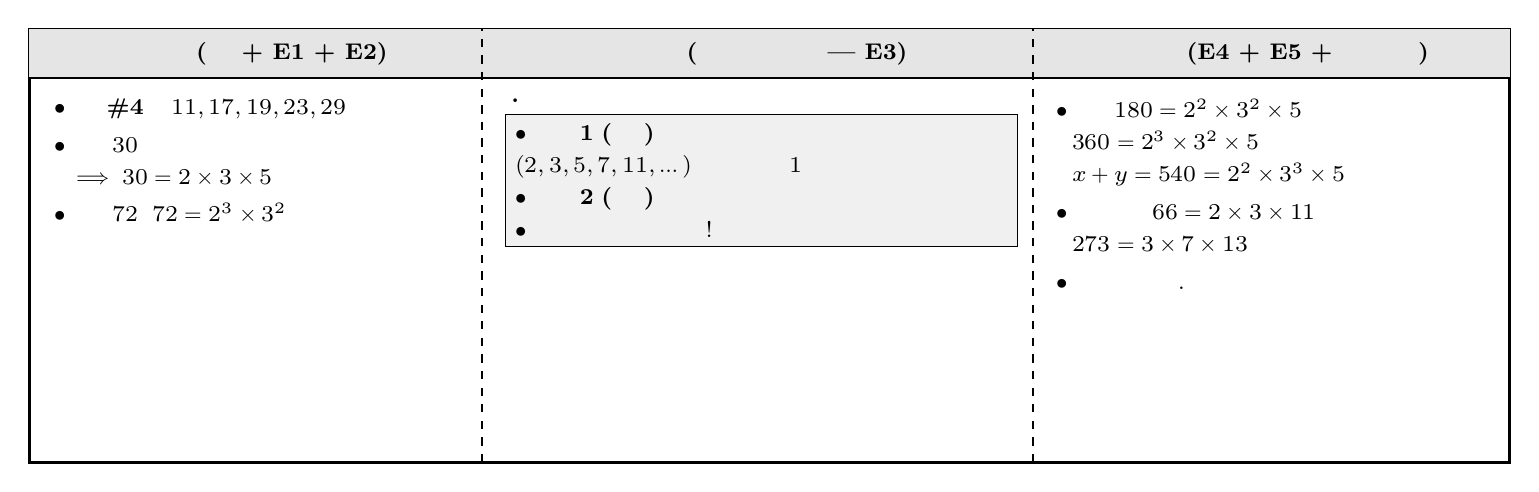
\begin{tikzpicture}[x=1cm, y=1cm, every node/.style={font=\fontsize{8.2pt}{11.6pt}\selectfont, text=black}]
  \draw[black, line width=1.1pt] (0,0) rectangle (18.8,5.50);
  \fill[gray!20] (0,4.88) rectangle (18.8,5.50);
  \draw[black, line width=0.7pt] (0,4.88) -- (18.8,4.88);
  \draw[black, dashed, line width=0.7pt] (5.75,0) -- (5.75,5.50);
  \draw[black, dashed, line width=0.7pt] (12.75,0) -- (12.75,5.50);

  \node at (2.875,5.19) {\textbf{ផ្នែកឆ្វេង (កំណែ + \en{E1} + \en{E2})}};
  \node at (9.25,5.19) {\textbf{ផ្នែកកណ្ដាល (ខ្លឹមសារគោលរក្សាទុក — \en{E3})}};
  \node at (15.775,5.19) {\textbf{ផ្នែកស្ដាំ (\en{E4} + \en{E5} + កិច្ចការផ្ទះ)}};

  % Left
  \node[anchor=north west, text width=5.30cm] at (0.20,4.74) {%
    $\bullet$ \textbf{កំណែ \#4 ខ៖} $11, 17, 19, 23, 29$\\[2pt]
    $\bullet$ \textbf{បំបែក $30$៖} ចែកឈរ និងដើមឈើ\\
    \hspace*{0.2cm}$\implies 30 = 2 \times 3 \times 5$\\[2pt]
    $\bullet$ \textbf{បំបែក $72$៖} $72 = 2^3 \times 3^2$
  };

  % Center
  \node[anchor=north west, text width=6.65cm] at (5.92,4.74) {%
    {\muol\fontsize{8.2pt}{11.8pt}\selectfont ៤\enbf{.} ការបំបែកជាផលគុណកត្តាបឋម}\\[3pt]
    \tikz\node[draw=black, fill=gray!12, inner sep=3.5pt, text width=6.25cm]{%
      $\bullet$ \textbf{វិធីទី 1 (ចែកឈរ)៖} ចែកបន្តបន្ទាប់នឹងបឋមពីតូចទៅធំ ($2, 3, 5, 7, 11, \dots$) រហូតផលចែកស្មើ $1$\\
      $\bullet$ \textbf{វិធីទី 2 (ដើមឈើ)៖} បែកមែករហូតគ្រប់ចុងមែកសុទ្ធតែជាចំនួនបឋម\\
      $\bullet$ សរសេរជាស្វ័យគុណតាមលំដាប់កើន!
    };
  };

  % Right
  \node[anchor=north west, text width=5.65cm] at (12.92,4.74) {%
    $\bullet$ \textbf{គំរូ៖} $180 = 2^2\times 3^2\times 5$\\
    \hspace*{0.2cm}$360 = 2^3\times 3^2\times 5$\\
    \hspace*{0.2cm}$x+y = 540 = 2^2\times 3^3\times 5$\\[2pt]
    $\bullet$ \textbf{ប្រតិបត្តិ៖} $66 = 2\times 3\times 11$\\
    \hspace*{0.2cm}$273 = 3\times 7\times 13$\\[2pt]
    $\bullet$ \textbf{កិច្ចការផ្ទះ៖} ទំ.២៤ លេខ ៥
  };
\end{tikzpicture}
\end{center}

\vfill
\secstrip{២. ចម្លើយផ្ទៀងផ្ទាត់រហ័សសម្រាប់សន្លឹកកិច្ចការសិស្ស \enbf{(}ទំព័រ ១ និង ទំព័រ ២\enbf{)}}{\en{Answer Key}}

\begin{tcolorbox}[
  enhanced, sharp corners, colback=white, colframe=black,
  boxrule=0.8pt, boxsep=2.5pt, top=4pt, bottom=4pt, left=6pt, right=6pt
]
  \fontsize{8.8pt}{13.0pt}\selectfont
  $\bullet$ \textbf{ផ្នែក \en{E1}៖} \textbf{សិស្ស ខ} ត្រឹមត្រូវ ($36 = 2^2\times 3^2$) ។ \textbf{ផ្នែក \en{E2}៖} \en{E2-A}: $30 = 2\times 3\times 5$; \en{E2-B}: $36 \to 18 \to 9 \to 3 \to 1 \implies 72 = \mathbf{2^3\times 3^2}$ ($8\times 9=72$) ។\\[2pt]
  $\bullet$ \textbf{ផ្នែក \en{E4}៖} ក. $180 = \mathbf{2^2\times 3^2\times 5}$, $360 = \mathbf{2^3\times 3^2\times 5}$ ។ ខ. $x+y=540 = \mathbf{2^2\times 3^3\times 5}$ ។ \en{EIA}៖ គុណគោលដូចគ្នា ។\\[2pt]
  $\bullet$ \textbf{ផ្នែក \en{E5}៖} ១) ក. $66 = \mathbf{2\times 3\times 11}$; ខ. $273 = \mathbf{3\times 7\times 13}$ ។ ៣) \textbf{ជម្រើស \en{B}} ។ ៤) សំបុត្រចេញ៖ $90 = \mathbf{2\times 3^2\times 5}$ ។
\end{tcolorbox}

\vfill
\secstrip{៣. ចម្លើយលម្អិតនៃកិច្ចការផ្ទះ \enbf{(}សៀវភៅគោល ទំ.២៤ លេខ ៥ ទាំង ៩ ចំនួន\enbf{)}}{សៀវភៅគោល ទំ.២៤}

\begin{tcolorbox}[
  enhanced, sharp corners, colback=white, colframe=black,
  boxrule=0.8pt, boxsep=2.5pt, top=4pt, bottom=4pt, left=6pt, right=6pt
]
  \fontsize{8.6pt}{12.7pt}\selectfont
  $\bullet$ $63 = \mathbf{3^2 \times 7}$ \quad $\mid$ \quad $100 = \mathbf{2^2 \times 5^2}$ \quad $\mid$ \quad $129 = \mathbf{3 \times 43}$ ($43$ បឋម) \quad $\mid$ \quad $225 = \mathbf{3^2 \times 5^2}$ \quad $\mid$ \quad $567 = \mathbf{3^4 \times 7}$ ($81\times 7$)\\[2.5pt]
  $\bullet$ $1\,980 = \mathbf{2^2 \times 3^2 \times 5 \times 11}$ \quad $\mid$ \quad $2\,097 = \mathbf{3^2 \times 233}$ ($2\,097\div 9 = 233$ ជាចំនួនបឋម!)\\[2.5pt]
  $\bullet$ $50\,336 = 32 \times 1\,573 = \mathbf{2^5 \times 11^2 \times 13}$ \quad $\mid$ \quad $127\,008 = 32 \times 3\,969 = \mathbf{2^5 \times 3^4 \times 7^2}$ ។
\end{tcolorbox}

\vfill
\secstrip{៤. ចំណុចប្រុងប្រយ័ត្នគរុកោសល្យសម្រាប់គ្រូ \enbf{(}គន្លឹះបំបែកចំនួនធំៗក្នុងលំហាត់ លេខ ៥\enbf{)}}{\en{Pedagogical Watchlist}}

\begin{tcolorbox}[
  enhanced, sharp corners, colback=panelgray, colframe=black,
  boxrule=0.85pt, boxsep=2.5pt, top=4pt, bottom=4pt, left=6pt, right=6pt
]
  \fontsize{8.6pt}{12.6pt}\selectfont
  $\bullet$ \textbf{ចំនួនធំ $50\,336$៖} ចែកនឹង $2$ ចំនួន $5$ ដងបាន $1\,573$ ។ ពិនិត្យ $1\,573$ ឃើញមិនចែកដាច់នឹង $2, 3, 5, 7$ តែចែកដាច់នឹង $11$៖ $1\,573\div 11 = 143 = 11\times 13$!\\[2pt]
  $\bullet$ \textbf{ចំនួន $2\,097$៖} ចែកដាច់នឹង $9$ ($2+0+9+7=18$) បាន $233$ ។ ពិនិត្យបឋម $\le 15$ ($2, 3, 5, 7, 11, 13$ — ព្រោះ $17^2=289>233$) ឃើញ $233$ មិនចែកដាច់នឹងមួយណាសោះ ដូច្នេះ $233$ ជាចំនួនបឋម!
\end{tcolorbox}

\end{document}
